%% TeX-command-extra-options: "-shell-escape"
\documentclass[11pt]{article}
\usepackage[utf8]{inputenc}
\usepackage[T1]{fontenc}
\usepackage{grffile}
\usepackage{longtable}
\usepackage{wrapfig}
\usepackage{rotating}
\usepackage[normalem]{ulem}
\usepackage{amssymb,amsmath,amsthm}
\usepackage{textcomp}
\usepackage{amssymb}
\usepackage{capt-of}
\usepackage{hyperref}
\hypersetup{colorlinks=true, linkcolor=magenta, citecolor=cyan}
\setlength{\parindent}{0in}
\usepackage[margin=1in]{geometry}
\usepackage[english]{babel}
\usepackage{mathtools}
\usepackage{palatino}
\usepackage{fancyhdr}
\usepackage{sectsty}
\usepackage{engord}
\usepackage{parskip}
\usepackage{graphicx}
\usepackage{subcaption}
\usepackage{setspace}
\usepackage{placeins}
\usepackage{color}
\usepackage{float}
\usepackage{bm}
\usepackage{pdfpages}
\usepackage{natbib}
\usepackage[ruled,vlined]{algorithm2e}
\usepackage{tikz}
\usetikzlibrary{bayesnet}
\usepackage{graphicx} % Inclusión de imágenes.
\usepackage{grffile}  % Distintos formatos para imágenes.
\usepackage{longtable} % Tablas multipágina.
\usepackage{wrapfig} % Coloca texto alrededor d

\theoremstyle{definition}

% Tikz
\usepackage{tikz}
\usetikzlibrary{positioning}
\usetikzlibrary{bayesnet}
\usetikzlibrary{shapes.geometric}
\usetikzlibrary{decorations.text}

\author{Luis Antonio Ortega Andrés}
\date{\today}
\title{Bayesian methods \\ \large Exam Questions and Solutions}

\DeclareMathOperator*{\argmin}{arg\,min} % thin space, limits underneath in displays
\DeclareMathOperator*{\argmax}{arg\,max} % thin space, limits underneath in displays

\newcommand*{\QED}{\null\nobreak\hfill\ensuremath{\square}}%

\begin{document}

\maketitle

\textbf{Exercise 1. }\emph{Consider a biased coin with unknown probability of heads \( \theta \). After \( N \)  tosses, we get \( K \)  heads and \( L \)  tails. Comment about the differences between maximum likelihood estimation and Bayesian estimation for computing the probability of heads for the next toss.}

On the one hand, maximum likelihood estimation derives a predictive probability that equals the empirical distribution, that is 
\[
     P( X = \text{heads}) = \frac{K}{N}.
\]
This approach presents two main disadvantages:
\begin{enumerate}
    \item Assigns zero probability to events that are not between the observations. For example, if \( N = L = 4 \), the probability of heads is zero.
    \item Does not take in to account the number of samples, just the proportion. That is, we may assign a heads probability of \( 0.5 \) with \( K = 1, N = 2 \) and \( K = 1000, N = 2000\).  
\end{enumerate}

These two issues are well handled with a Bayesian approach with a proper prior definition. For example, given the nature of the parameter, we might consider a Beta distribution as prior knowledge \( P(\theta) = Beta(\alpha, \beta) \propto \beta^{\alpha - 1}(1 - \theta)^{\beta - 1} \). Given that conjugacy holds, the posterior probability is
\[
    \begin{aligned}
    P(\theta \mid \bm{x}) &\propto P(\bm{\theta} \mid \theta)P(\theta) = \prod_n P(x_n \mid \theta)P(\theta) \propto \theta^{\ \alpha + K - 1}(1-\theta)^{\beta + L - 1} \\
    &= Beta(\alpha + K, \beta + L).
    \end{aligned}
\]
With a predictive posterior of \( P(x^{new} \mid \theta, \bm{x}) = \mathbb{E}[P(\theta \mid \bm{x})]\). The main disadvantage of a Bayesian approach is that it requires prior knowledge over the problem, given that uninformative prior might lead to non accurate results.  

\textbf{Exercise 2. }\emph{Consider the following distribution}
\[
     P(A,B,C,D,E,F,G) = P(A)P(B)P(C \mid A, B)P(D \mid A, B, C)P(E \mid A, D)P(F \mid B, D)P(G \mid E).
\]
\emph{Answer the following questions:}
\begin{enumerate}
    \item \emph{Draw the Bayesian network associated with the given factorization.}
    \item \emph{Draw the moralized graph.}
    \item \emph{Draw the triangularized graph.}
    \item \emph{Obtain the cluster tree graph (or junction tree) and check that it fulfils the running intersection property.}
    \item \emph{Obtain all the messages of the tree.}
    \item \emph{Check that the marginal distribution of the cluster node with the highest number of variables obtained from the messages is equal to that obtained directly by marginalizing the above formula. Compute the messages in the proper order.}
\end{enumerate}

\begin{enumerate}
    \item Bayesian network.
    \begin{figure}[H]
        \centering
    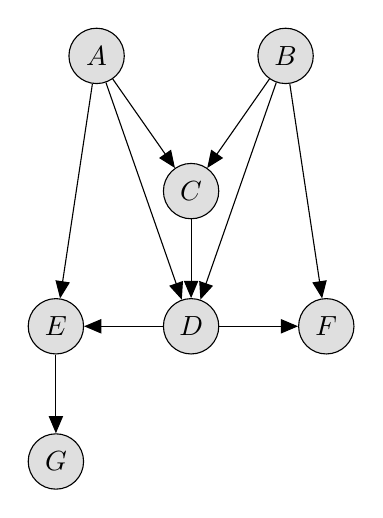
\begin{tikzpicture}
    
        % Define nodes
        \node[obs]                            (c) {$C$};
        \node[obs, above=of c, xshift=-1.2cm] (a) {$A$};
        \node[obs, above=of c, xshift=1.2cm]  (b) {$B$};
        \node[obs, below=of c]                (d) {$D$};
        \node[obs, right=of d]                (f) {$F$};
        \node[obs, left=of d]                 (e) {$E$};
        \node[obs, below=of e]                 (g) {$G$};
        % Connect the nodes
        \edge {a,b} {c}; %
        \edge {a,b, c} {d}; %
        \edge {a, d} { e};
        \edge {b,d} {f};
        \edge {e} {g};
    
      
      \end{tikzpicture}
    \end{figure}
    \item The moralized graph consists in the undirected graph that results on adding edges between parents of the same child. 
    \begin{figure}[H]
        \centering
    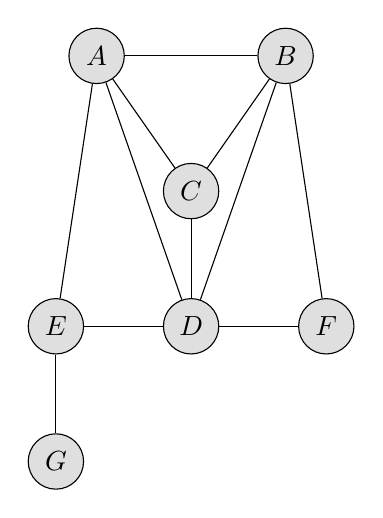
\begin{tikzpicture}
    
        % Define nodes
        \node[obs]                            (c) {$C$};
        \node[obs, above=of c, xshift=-1.2cm] (a) {$A$};
        \node[obs, above=of c, xshift=1.2cm]  (b) {$B$};
        \node[obs, below=of c]                (d) {$D$};
        \node[obs, right=of d]                (f) {$F$};
        \node[obs, left=of d]                 (e) {$E$};
        \node[obs, below=of e]                 (g) {$G$};
        % Connect the nodes
        \edge[-] {a}{b};
        \edge[-] {a,b} {c}; %
        \edge[-] {a,b, c} {d}; %
        \edge[-] {a, d} { e};
        \edge[-]  {b,d} {f};
        \edge[-] {e} {g};
      \end{tikzpicture}
    \end{figure}
    \item The triangulated graph consists on triangulating any loop of \( 4 \) or more vertices. In this case, no change is needed.
    \item In order to build the associated junction tree, we need every maximal clique, i.e, cliques that are not contained in any other clique. In this case \( (A,B,C,D), (B,D,F), (A,E,D) \) and \( (E,G) \). The junction tree is created by adding edges between these subsets without making any loops.
    \begin{figure}[H]
        \centering
    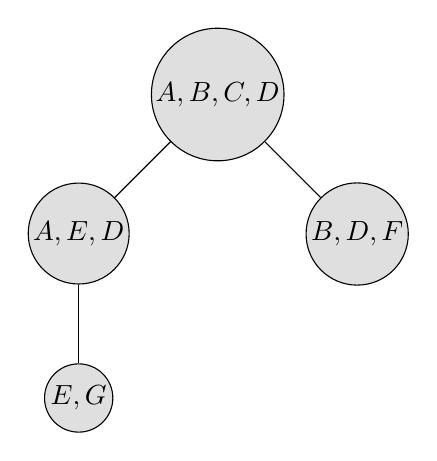
\begin{tikzpicture}
    
        % Define nodes
        \node[obs]                (1) {$A,B,C,D$};
        \node[obs, below right=of 1]    (2) {$B,D,F$};
        \node[obs, below left=of 1]    (3) {$A,E,D$};
        \node[obs, below=of 3]      (4) {$E,G$};

        % Connect the nodes
        \edge[-] {1}{2};
        \edge[-] {1}{3};
        \edge[-] {3}{4};
      \end{tikzpicture}
    \end{figure}
    The associated factors are:
    \[
        \begin{aligned}
            (A, B, C, D) &\to \psi_1 = P(A)P(B)P(C\mid A, B)P(D \mid A, B, C)\\
            (A, E, D) &\to \psi_2 = P(E \mid A, D)\\
            (B, D, F) &\to \psi_3 = P(F \mid B, D)\\
            (G, E) &\to \psi_4 = P(G \mid E)
        \end{aligned}
    \]
    \item Each node messages are 
    \[
        \begin{aligned}
        \end{aligned}
    \]
\end{enumerate}



\textbf{Exercise.} \emph{Assume you are given an un-normalized probability distribution that has the following factors (potentials): \( \phi(A,B)\phi(B,C)\phi(C,D)\phi(D,A) \). Draw a valid cluster graph that is not a tree on which to run loopy belief propagation and explain the advantages and disadvantages of running loopy belief propagation on non-tree graphs when compared to running belief propagation on a cluster graph that is a tree.}

We might consider Bethe Cluster Graph:
\begin{figure}[H]
    \centering
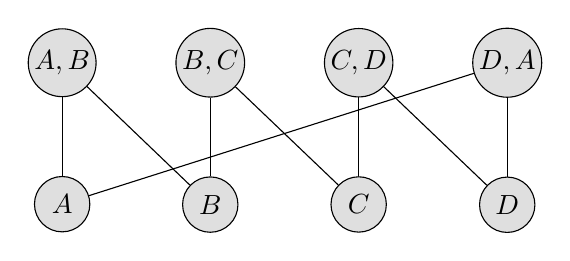
\begin{tikzpicture}

    % Define nodes
    \node[obs]               (ab) {$A,B$};
    \node[obs, right=of ab]  (bc) {$B,C$};
    \node[obs, right=of bc]  (cd) {$C,D$};
    \node[obs, right=of cd]  (da) {$D,A$};
    \node[obs, below=of ab]  (a) {$A$};
    \node[obs, below=of bc]  (b) {$B$};
    \node[obs, below=of cd]  (c) {$C$};
    \node[obs, below=of da]  (d) {$D$};

    % Connect the nodes
    \edge[-] {a,b} {ab}; %
    \edge[-] {c,b} {bc}; %
    \edge[-] {c,d} {cd}; %
    \edge[-] {d,a} {da}; %
  \end{tikzpicture}
\end{figure}

The main disadvantage of running Belief Propagation on a cluster graph is that its cost is exponential in the size of the scope of the largest factor. When the largest node is to big, exact computations might be intractable, leading to the need of approximate methods, as Loopy Belief Propagation.

The main disadvantage of Loopy Belief Propagation is that messages are approximated and it is not guaranteed to converge (which might be solved via message dampening).

It is worth mentioning that Bethe's cluster graph simplifies finding a graph for LPB, whilst there is no equivalent graph for exact BP.

\textbf{Exercise. }\emph{Describe message damping or smoothing in loopy belief propagation and indicate its main utility}.

Message damping is a technique that is used in Loopy Belief Propagation to improve its convergence. The idea is to set the messages as a combination of the previous message and the new one
\[
     \delta^{new}_{i,j} = \lambda\left( \sum_{C_i - S_{i,j}} \psi_i \prod_{k \in Neig_i - j} \delta_{k,i} \right) + (1-\lambda)\delta_{i,j}^{old}.
\]
This avoids strong changes in the messages and helps convergence. The parameter \( \alpha \in [0,1] \) controls the amount of used dampening. 


\textbf{Exercise. }\emph{ Consider an un-normalized distribution \( P(A, B) \)  over two discrete variables \( A \)  and \( B \). Explain how to obtain the corresponding mean-field approximation to that distribution. Recall that mean-field is a particular case of variational inference.}

Under the mean field approximation we find a distribution \( Q \) that approximates the un-normalized target distribution. The main assumption made is that \( Q \) factorizes in some manner. In this case \( Q(A, B) = Q(A)Q(B) \). The optimal factors are found by minimizing the Kullback-Leibler divergence between \( Q \) and the target distribution, or equivalently, by maximizing the lower bound of the marginal likelihood. In particular, under the assumption that the first factor \( Q(A) \)  is fixed, \( \mathcal{L}(Q) \) is maximized with respect to the second factor \( Q(B) \) and conversely, creating an iterative procedure.

\textbf{Exercise. }\emph{Explain how to use expectation propagation to approximate an un-normalized distribution of the following form: \( f_1(z)f_2(z\mathcal{N}(z \mid \mu, \sigma^2)) \), where the first two factors are non-Gaussian and \( \mu,\sigma^2 \) are known. Assume that the approximate distribution \( Q \) is Gaussian.}

In EP all factors that do not lie in the family of the approximating distribution are projected to that family by minimizing the reverse KL divergence. In this case, the factors \( f_1 \) and \( f_2 \) will be approximated by Gaussian factors \( \bar{f}_1 \) and \( \bar{f_2} \). Each approximate factor will be updated via a iterative procedure:
\begin{enumerate}
    \item Compute \( Q^{\backslash i} = Q / \bar{f}_i \).
    \item Update the approximating distribution by minimizing \( KL\left(\frac{1}{Z}Q^{\backslash i} f_i \mid Q\right) \) over \( Q \). This is done by \emph{moment matching}, i.e,  matching their expected sufficient statistics. 
    \item Compute the new factor \( \bar{f}_i^{new} = Z \frac{Q}{Q^{\backslash i}} \).  
\end{enumerate}

The last factor does not need to be approximated as it is already Gaussian.

\textbf{Exercise. } \emph{Draw the Bethe cluster graph associated to the un-normalized distribution of the previous question and write the messages that will be exchanged between the nodes in the cluster graph when expectation propagation is considered as a generalization of belief propagation with approximate messages. Indicate which messages are exact and which messages are approximate}.

The resulting Bethe cluster is 
\begin{figure}[H]
    \centering
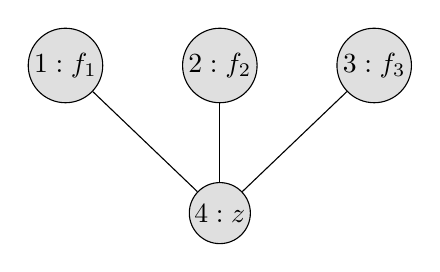
\begin{tikzpicture}

    % Define nodes
    \node[obs]               (ab) {$1: f_1$};
    \node[obs, right=of ab]  (bc) {$2: f_2$};
    \node[obs, right=of bc]  (cd) {$3: f_3$};
    \node[obs, below=of bc]  (b) {$4: z$};


    % Connect the nodes
    \edge[-] {b} {ab}; %
    \edge[-] {b} {bc}; %
    \edge[-] {b} {cd}; %
  \end{tikzpicture}
\end{figure}
Where the messages are:
\[
     \begin{aligned}
        \delta_{4,1} &= Q/f^1 \quad \text{exact message.}\\
        \delta_{4,2} &= Q/f^2\quad \text{exact message.}\\
        \delta_{4,3} &= Q/\mathcal{N}(z \mid \mu, \sigma^2)\quad \text{exact message.}\\
        \delta_{1,4} &= \bar{f}_1\quad \text{approximate message.}\\
        \delta_{2,4} &= \bar{f}_2\quad \text{approximate message.}\\
        \delta_{3,4} &= \mathcal{N}(z \mid \mu, \sigma^2)\quad \text{exact message.}\\
     \end{aligned}
\]


\end{document}